As we have seen before, MALIS performs really well, but can still be
improved.\\
It was most notably improved in~\cite{funke_large_2019} where they were able to
improve the affinity prediction using more recent architectures, by improving
the training and taking full advantage of the MST and by applying a
post-processing on the affinity graph instead of a simple thresholding.

\begin{figure}[!htbp]
	\centering
	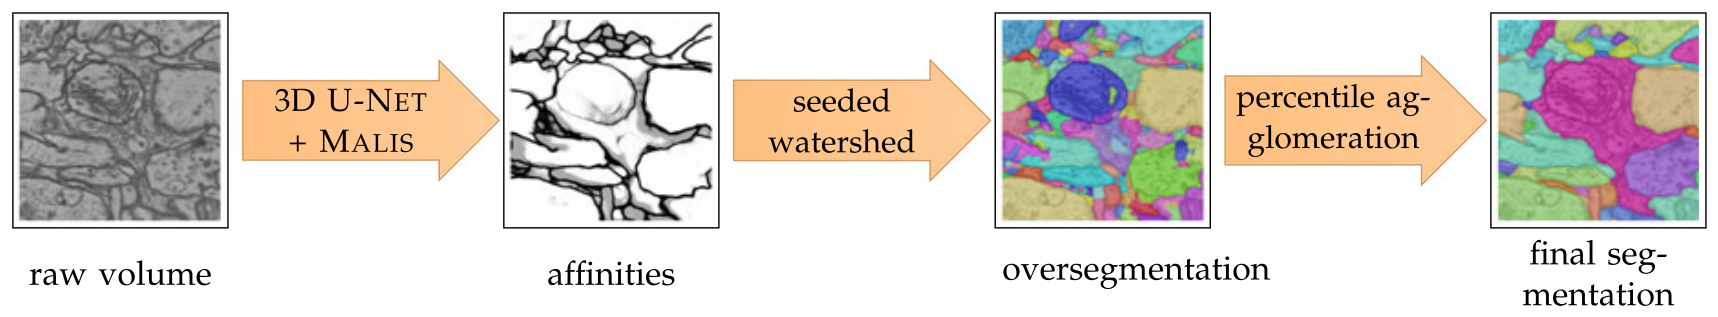
\includegraphics[width=0.8\linewidth]{./images/mala_process.png}
	\caption{Improves MALIS as described in~\cite{funke_large_2019}}%
	\label{fig:mala_process}
\end{figure}

As we can see in figure~\ref{fig:mala_process} the CNN was replaced by a U-Net,
which we will describe afterwards. Then the segmentation is obtained using a
seeded-watershed, which is then improved using a percentile agglomeration of
small objects.

\subsection{Using a more potent architecture}
Indeed, one of the limits of the previous method was the use of a relatively
simple neural network to predict the affinity. This is mostly due to the fact
that neural networks have greatly improved since the original
paper~\cite{turaga_maximin_2009} in 2009.\\

\begin{figure}[!htbp]
	\centering
	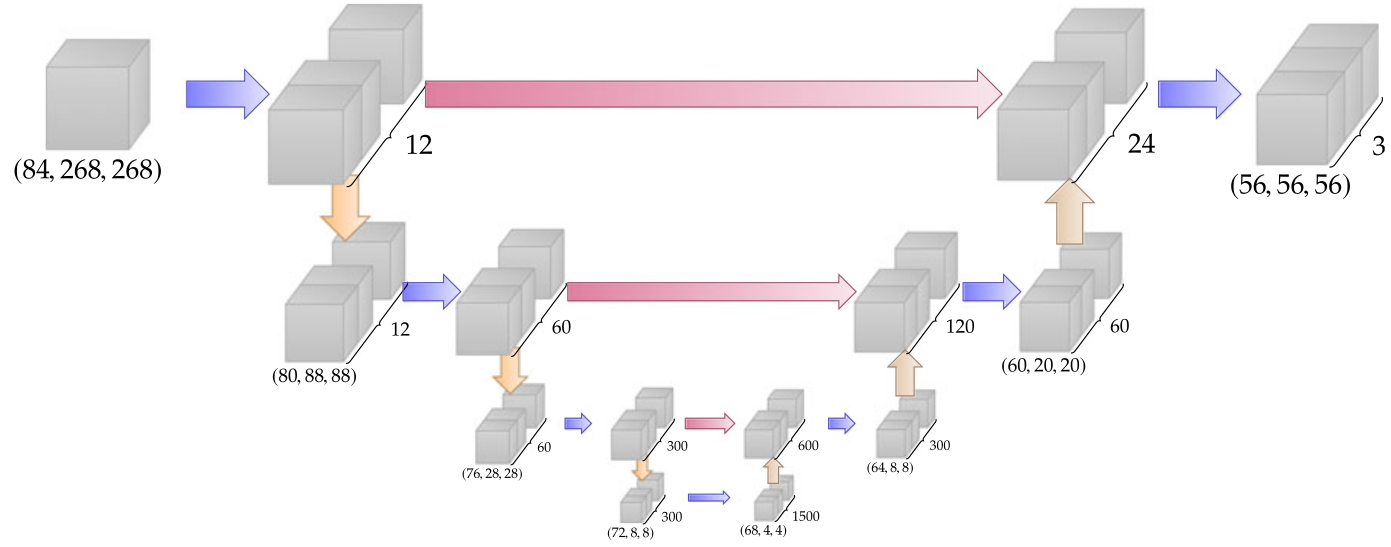
\includegraphics[width=0.8\linewidth]{./images/mala_architecture.png}
	\caption{U-Net architecture used on the CREMI dataset from~\cite{funke_large_2019}}%
	\label{fig:mala_unet}
\end{figure}


U-nets especially have been widely used for image segmentation and are thus a
natural choice in our case. The architecture used in~\cite{funke_large_2019}
is shown in figure~\ref{fig:mala_unet}. As we can see, the training will
obviously be much longer than previously, but the results should be
significantly better.\\
A question that can arise is why not simply use just a U-Net without the MALIS
loss, and as we will see later, the MALIS loss gives us better results on
differents measures of segmentation quality.


\subsection{Constrained MALIS loss}

Previously, we only computed the maximin edge for a pair of pixels (or a finite
amount of pairs), which means that some information from the MST was not
used.\\
However, we would like to compute the maximin edge for all pairs of pixels in
the image. This was not done in the previous paper for time efficiency
reasons.\\
However they describe a way to compute the loss with in quasilinear time instead
of in polynomial time.\\

The main idea is that all maximin edges are in the MST, and there are $n-1$
edges if we have $n$ pixels in our image. We could then simply compute the loss
over all those edges but this would mean that they are all as important as the
others. However since we have $n^2$ pairs of points and $n-1$ edges in our MST,
they will be the maximin edge for a different number of pixel-pairs. So we must
find a way to see how often an edge from the MST is a maximin edge.\\

When we add an edge using Kruskal's algorithm, we can look at the "size" of the
trees it merges and deduce the number of pairs for which the current edge is
the maximin edge.\\

From this, we can define the positive weight of an edge $e$ as the number of pairs
from the same object/segment merged by adding $e$ to the MST. More formally we
have :
\begin{equation*}
	w_p(e)=\lvert \{(u,v)\in F^2 \;|\;\delta(u,v)=1, e=mm(u,v) \}   \rvert
\end{equation*}

Similarly we can define the negative weight of an edge as :
\begin{equation*}
	w_n(e)=\lvert \{(u,v)\in F^2 \;|\;\delta(u,v)=0, e=mm(u,v) \}   \rvert
\end{equation*}

These formulations allow us to rewrite our loss function as :

\begin{equation*}
	L(I,\theta,S) = \sum_{e\in MST(G)} w_p(e)l(1,A_e(I,\theta)) + w_nl(0,A_e(I,\theta))
\end{equation*}
With $A_e$ the affinity of an edge $e$.\\

The idea to compute $w_n$ and $w_p$ is that every time that an edge $e$ is
added to our MST, it merges two trees $T_1$ and $T_2$.\\
We will define $V_{T_i}$ as the set of vertices in the tree $i$.
If we take two pixels $i \in V_{T_1}$ and $j \in V{T_2}$ we can be sure that $e$ is
their maximin edge, as it is the edge with lowest affinity in the path from $i$
to $j$. \\
As such we can already deduce that there are $|T_1||T_2|$ pairs of
pixels with $e$ as their maximin edge, but we don't know yet for which of these
pairs if they should be in the same object or not, which is necessary to
compute $w_n$ and $w_p$.\\

To do so we need to not only keep track of the areas when computing our MST,
which is straigthforward, but also keep track of areas per label.\\
To get the area per label when adding an edge, we can simply add together the
areas per label from both trees that are merged by this edge.\\

By defining $V_{T_i}^j$ as the set of vertices in tree $T_i$ with label $j$, we
can compute $w_n$ and $w_p$ as follows: 

\[
	w_p(e) = \sum_{i\in{1\ldots k}} \lvert V_{T_1}^i \rvert \lvert V_{T_2}^i \rvert
\]
\[
	w_n(e) = \sum_{i\neq j \in{1\ldots k}} \lvert V_{T_1}^i \rvert \lvert
	V_{T_2}^j \rvert = \lvert V_{T_1} \rvert \lvert V_{T_2} \rvert - w_p(e)
\]

Since this is computable in $\mathcal{O}(k)$ and we need to to this step $n$
times, the added complexity is only in $\mathcal{O}(kn)$, making the total
computation of the loss in $\mathcal{O}(n\text{log}(n) + kn)$.\\

With this loss function being able to be computed in quasilinear time, this
will allow us to use the whole patch for the loss computation instead of a few
pairs of pixels, which should improve the results. This loss function is the
same as before, it still is related to the Rand Index, but it should now
approximate it much better.\\

\subsection{Two pass computation of the loss}

An issue with the aforementioned loss is that all edges have both a positive
weight, where we will compare them to the value 1 and a negative weight where
we will compare them to 0.\\

However an edge as an optimal value of either 1 or 0, not both, so how can we
only take only into account the right value ?

\begin{figure}[!htpb]
	\centering
	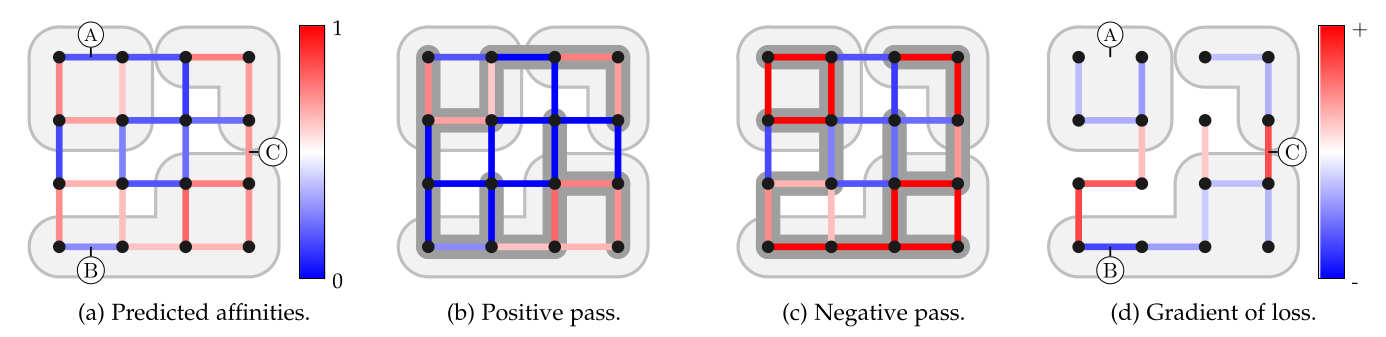
\includegraphics[width=1\linewidth]{./images/two_pass.png}
	\caption{Illustration of the constrained MALIS loss, blue edges represent a
	low affinity and red edges a high affinity; from~\cite{funke_large_2019}}%
	\label{fig:two-pass}
\end{figure}

As we can see in figure~\ref{fig:two-pass}, we will compute the loss in two
passes.
In the positive pass, (b), affinities of edges between ground-truth regions are
set to zero (blue), in the negative pass (c), affinities within ground-truth
regions are set to one (red). In either case, a maximal spanning tree (shown as
shadow) is constructed to identify maximin edges. Note that, in this example,
edge A is not a maximin edge in the positive pass since the incident voxels are
already connected by a high affinity path. In contrast, edge B is the maximin
edge of the bottom left voxel to any other voxel in the same region and thus
contributes to the loss. Similarly, C is the maximin edge connecting voxels of
different ground-truth regions and contributes during the negative pass to the
loss. The resulting gradients of the loss with respect to each edge affinity is
shown in (d) (positive values in red, negative in blue).\\

To really see the benefit we need to look at how each pass influences the loss
function. In the positive pass, since we set all negative edges (edges between
objects) to 0, their contribution to the loss will be 0, so the loss can be
rewritten as :
\begin{equation*}
	L(I,\theta,S) = \sum_{e\in MST(G)} w_p(e)l(1,A_e(I,\theta))
\end{equation*}

But can those negative edges have a non zero $w_p$ ?\\
Inside an object, we will have weights having a non zero value, or at worst
having value 0. So if we take $i,j$ in the same object, there will be a maximin
path that stays in this object, so no negative edge is the maximin edge for any
pair of pixel inside the same object, giving all of our negative edges a
positive weight equal to zero.\\
As such during the positive pass we only take into account the positive edges
(edges inside the same object) and their positive weight, which is exactly what
we wanted.\\

We will do similarly during the negative pass, where we will only take into
account the negative weight of negative edges.\\

Using these two passes we are able to only account for the useful terms inside
this loss, and overall achieve a more accurate loss than before.\\
The only issue with the two passes is the computation time. Although it doesn't
change the complexity, doing two passes doubles the time required to compute
the loss. However this is still far superior than the first formulation of the
loss, or the version in $\mathcal{O}(n^2)$.


\subsection{Seeded watershed as post processing}

Remember that before, we computed the segmentation by thresholding our affinity
graph. However this doesn't give optimal results, as for example locally
another threshold would perform better.\\
An issue that was also encountered was small objects that were inside bigger
ones. These objects lead to an oversegmentation and we would like a way to
automatically remove those inaccuracies, or at least part of them.

\begin{figure}[!htbp]
	\centering
	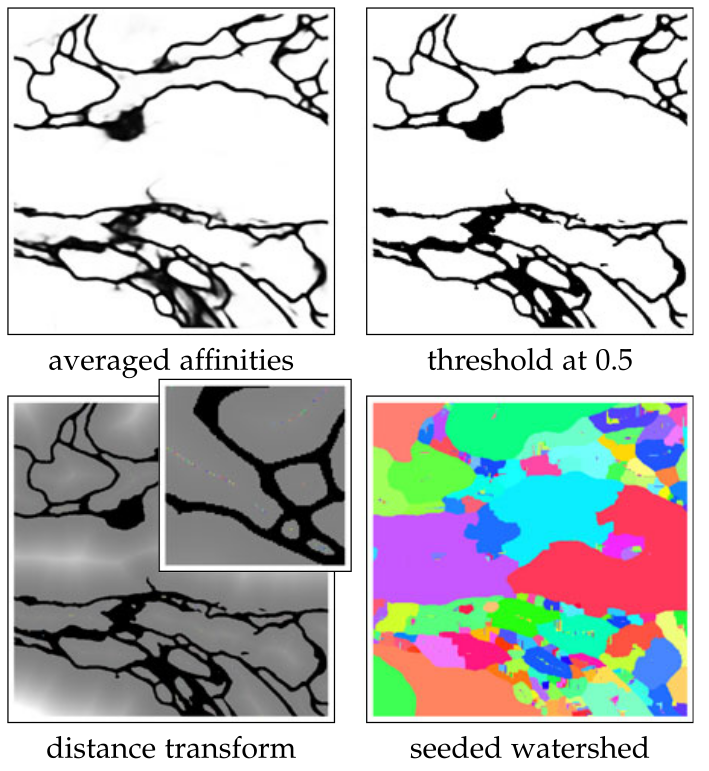
\includegraphics[width=0.5\linewidth]{./images/mala_post_proc.png}
	\caption{Seeded watershed on an affinity graph, as described in~\cite{funke_large_2019}}%
	\label{fig:seeded_ws}
\end{figure}

This is where the framework described in~\cite{funke_large_2019} comes in play.
As we can see in figure~\ref{fig:seeded_ws}, the first step of the process is
to average the affinities, as we did before. Afterwards the averaged affinities
are thresholded at 0.5 (here this threshold is not a parameter). Then a
distance transform (or a distance map) is computed from the objects to the
borders. In this distance transform, the furthest points from the borders will
have the higher values. Then, all the local maxima are taken as seeds for a
seeded watershed, which gives us a first segmentation.\\

This is still an oversegmentation, but a fragment agglomeration algorithm is
then used to fuse regions together. multiple criteria can be used to
determine which regions to merge together and they are described
in~\cite{funke_large_2019}.\\
When all of those steps are done, we obtain the final segmentation.\\

\textbf{\textcolor{red}{Describe agglomeration}}
\\

As we can see the process is greatly improved from the first version of MALIS,
with the loss function, the neural network architecture and the post processign
used being much more powerful than their previous counterparts.
